\section{Compiler Architecture}

\subsection{Overview}
The figure below presents the general architecture of the Qoala compiler:

\begin{figure*}[ht]
    \centering
    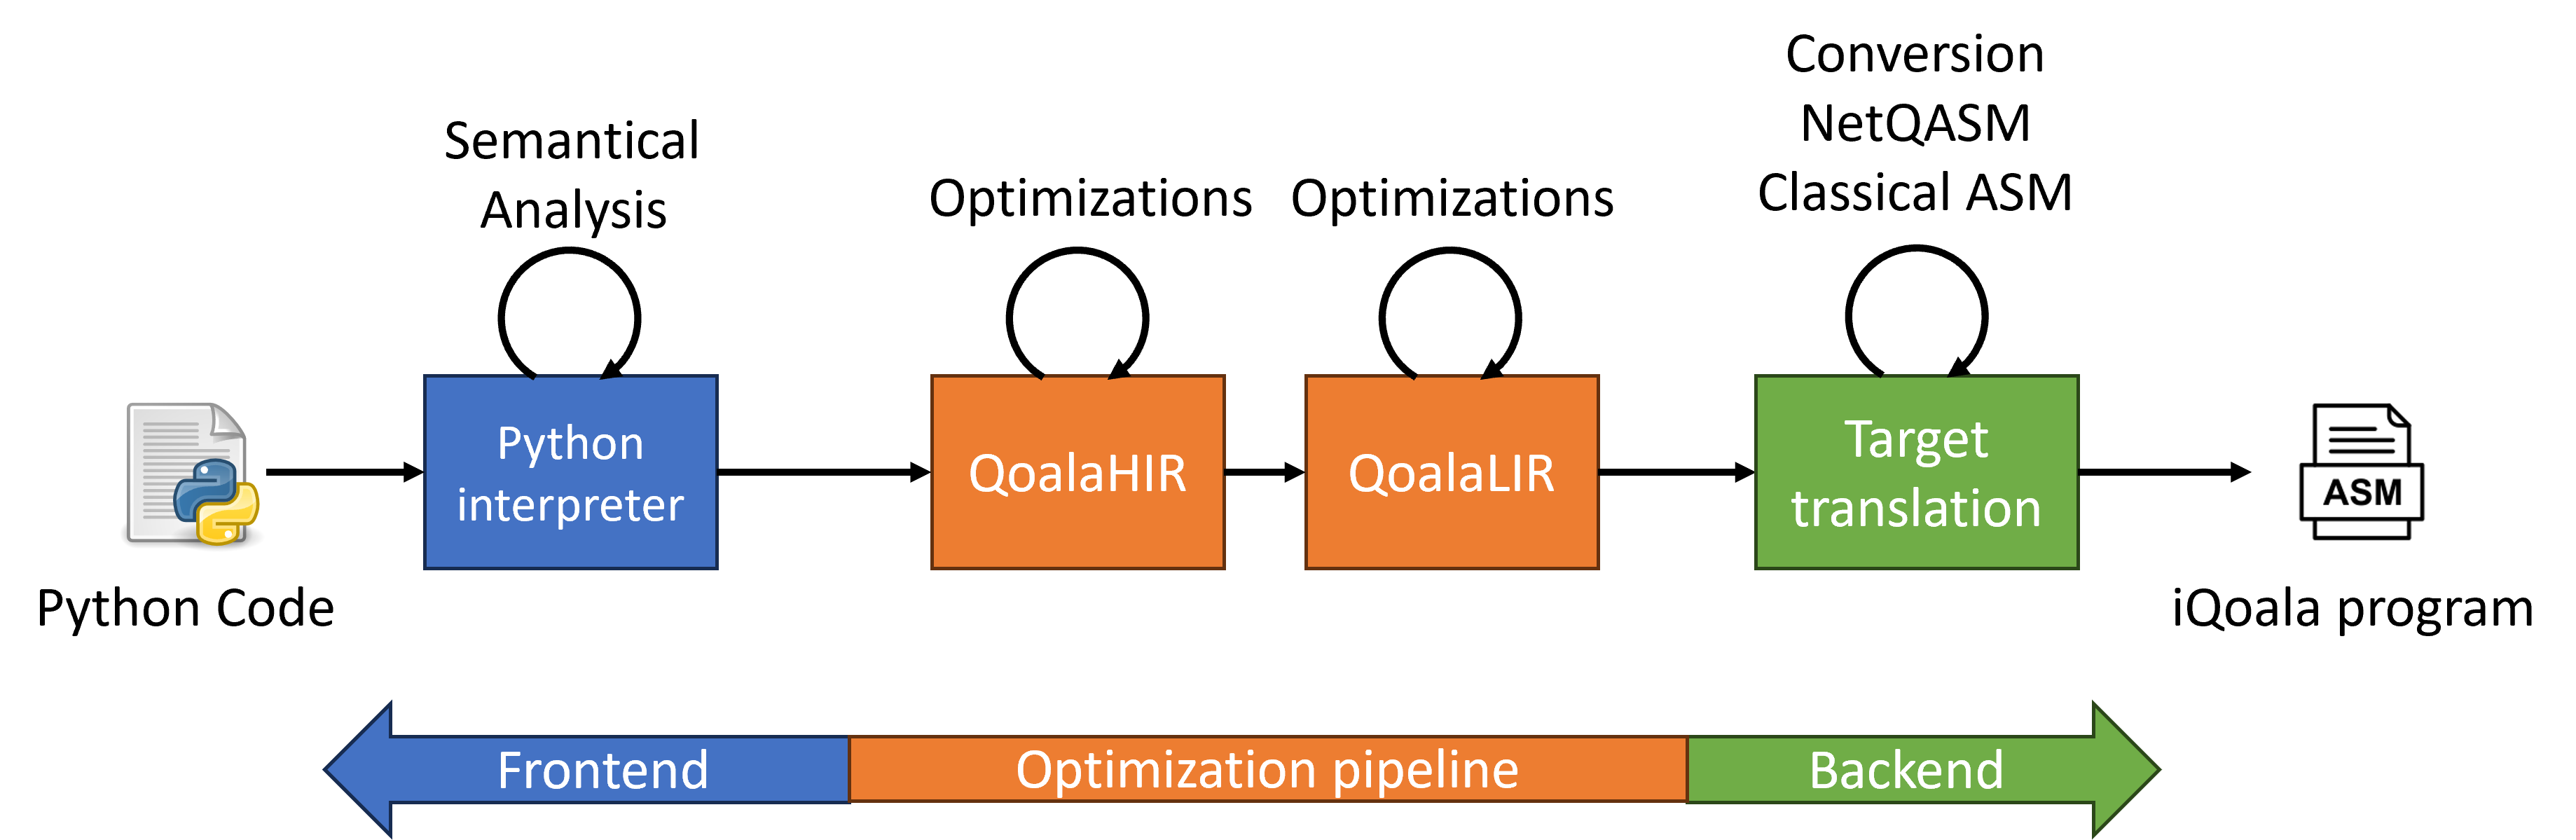
\includegraphics[scale=1.0]{figures/compiler/compiler-arch.png}
    \caption{Qoala compiler stages}
    \label{fig:qoala_compiler_stages}
\end{figure*}


The core steps in the Qoala compilation process are:

\begin{itemize}
\item Programmer writes source code in Python using the Qoala Python SDK.
\item The Python SDK itself provides a `compile` function that executes the source code
  which produces a `.mlir` file containing the program code in QoalaHIR format.
\item This Python SDK implements \textit{some} functionality present in the "frontend" of a classical
  compiler, for example, a semantical analysis to check the validity of the classical and
  quantum operations specified in the program 
\item A separate `opt`-like tool (built using LLVM/MLIR) takes the `.mlir` as input and produces
  (after several applying passes) a `.iqoala` file.
\item The `.iqoala` file can then be executed by a Qoala runtime.
\end{itemize}


\subsection{High-level choices}
\begin{itemize}
\item Why python
  Since it first launch, python was positioned as a programming language that allows the programmer to quickly develop
  solutions with less lines of code. Lowering the usual barriers from other programming language is what allowed python
  to gain popularity among the scientific community.
  The Qoala platform goes in this line by allowing the scientific community to write quantum internet programs in a
  language that is easy to use, that is easy to understand, and that is known by the scientific community.
\item Why MLIR
  MLIR is a modular and extensive compiler infrastructure that allows extending the LLVM infrastructure, easing the
  developing of domain-specific representations and allowing reusing other pieces of the LLVM compiler infrastructure.
  By allowing the definiton of \textit{dialects}, MLIR allows extending the intermediate representations of the clang compiler
  pipeline, enabling the conversion of programs between different dialects, and also alowing the re-usage of the
  optimizations and analysis implemented in other dialects.
  All these feature make MLIR a perfect candidate for creating the compiiler for hybrid quantum internet programs.
\item Why iqoala as output
\item Why protocol description
\end{itemize}
    

\subsection{Python SDK}
The Python SDK is a library containing classes and methods that allow:
- expressing quantum internet program logic, and
- producing a QoalaHIR representation of the source code

The general should look like this:

\begin{pycode}
class MyProgram(QoalaProgram):
    def main(self, ctx: QoalaContext):
        q = ctx.new_qubit()
        e = ctx.entangle_keep("Bob")
        ctx.cnot(q, e)
        m = ctx.measure(q)
        ctx.add_return(m)

program = MyProgram()
mlir = program.compile()  # `compile` is defined in `QoalaProgram`
with open("program.mlir", "w") as f:
    f.write(mlir.text())
\end{pycode}

The Python SDK acts as the "frontend" of the qoala compiler. In this sense,
the output of the Python SDK is a `.mlir` file in the QoalaHIR dialect.
By using Python as a the high-level language of the programs, we can take advantage
of the python interpreter to perform the parsing of the code and an initial
syntactical analysis.
To complete the frontend analysis, the Qoala libraries could also embed a
semantical analysis to check the correctness of the applied quantum operations.
As mentioned before, the main goal of this Python SDK (frontend) will be to
create a High Level representation of the program, using the QoalaHLIR
language, which will be the main input of the optimization pipeline int he next stages.


\subsection{MLIR-based optimizer pipeline}
The Qoala compiler also defines an optimization pipeline that analyses and
transforms the code to improve its performance and prepare it for the final
translation in the iQoala format.

To this end, the optimization pipeline makes use of the MLIR framework to
define intermediate representations as *dialects*. Later, the optimization
tools can apply *passes* on the intances of the program expressed using the
MLIR dialects.


\subsection{Representations and dialects}
The Qoala compiler uses three intermediate representations (IRs) when in the "MLIR-phase".
These are the High-level Intermediate Representation (HIR), Mid-level Intermediate Representation (MIR), and the Low-level Intermediate Representation (LIR).
Each IR is associated with a particular set of MLIR dialects.
The Qoala compiler uses four custom MLIR dialects, called `QNet`, `QMem`, `QoalaHost`, and `Netqasm`, explained in more detail below.

\begin{itemize}
\item HIR (High-level): A higher-level IR, where operations are closely related
  to the python source.
  Quantum operations are represented using the `QNet` dialect, which consume and produce quantum *values*.
  Programs in the HIR format use the following dialects: `QNet`, `arith`, `scf`, `affine`, `async`, `tensor`.
\item MIR (Mid-level): A mid level IR, similar to HIR but with explicit memory locations, using the `QMem` dialect instead of `QNet`.
\item LIR (Low-level): A lower level IR, where operations are closer to the
  classical and quantum assembly instructions.
  Quantum operations are represented using the `Netqasm` dialect, which take quantum *registers* ("quantum memory pointers") as operands
  and have side-effects on the quantum value stored in the registers.
  Programs in the LIR format use the following dialects: `QoalaHost`, `Netqasm`, `arith`, `scf`, `affine`, `async`.
\end{itemize}

Tranforming from HIR to LIR hence involves lowering QNet operations to QoalaHost and Netqasm operations.
On top of that, both HIR and LIR have additional constraints about the structure of code in that representation which need to be respected.



\begin{itemize}
\item High-level MLIR Dialect (QoalaHIR)
    \begin{itemize}
        \item Hybrid classical-quantum
        \item No memory allocation
        \item Timing and fidelity annotations
        \item Entanglement as abstract operation
    \end{itemize}
\item Low-level MLIR Dialect (QoalaLIR)
    \begin{itemize}
        \item Explicit split between classical and quantum code
        \item Memory allocation
        \item Timing and fidelity annotations
        \item Entanglement as abstract operation
    \end{itemize}
\item Translation passes:
    \begin{itemize}
        \item HIR -> LIR
        \item Codegen LIR -> QoalaHost instructions
        \item Codegen LIR -> NetQASM
    \end{itemize}
\item Optimization passes:
    \begin{itemize}
        \item Memory mapping on quantum LIR
        \item Find best split between cLIR and qLIR when translating HIR -> LIR (can be pass on HIR before translation)
        \item Convert fidelity constraints into timing constraints
        \item Extract constraints from protocol description into HIR annotations
    \end{itemize}
\end{itemize}


\subsubsection{General optimization pipeline}
The MLIR optimization pipeline applies the folliwng operations:
\begin{itemize}
\item apply optimzation passes on the QoalaHIR code
\item transform QoalaHIR to QoalaLIR
\item apply optimzation passes on the QoalaLIR code
\item generate `.iqoala` code from QoalaLIR
\end{itemize}

This optimization pipeline introduce modifications in different levels of the process:
\begin{itemize}
\item At HIR level: operations can be re-order, respecting the restrictions specified
  [in the HIR specification document](dialects/HIR.md).
\item Conversion from HIT to LIR: High-level qubit allocations instructions are exploded
  into the lower-level qubit allocation operations, which includes allocation,
  initialization and value writing/reading.
\item At LIR level: operations belonging to the same local quantum functions are grouped
  into functions ("functionize") to aid the scheduling at runtime.
\end{itemize}


\subsection{Optimizations}
We consider the following optimizations:
\begin{itemize}
\item qubit mapping optimization (already exists)
\item gate-level optimization (already exists)
\item classical-quantum division (limit host-qnodeos communication and limit qubit lifetimes)
\item inserting deadlines to try and meeting timing and fidelity constraints
\end{itemize}


\subsubsection{Memory Alloc (i.e. Qbits allocation)}
- Entanglement move to memory qubti??
- Use/keep of subroutines in iqoala ??

Idea: try to stitch together separate functions/subroutines to get one circuit and apply standard circuit optimizations on it.
Does not really work: in general programs can have many different circuits at runtime depending on control-flow.

Maybe: first functionize, then check qptrs that are passed into/out of function calls? Then try to map these pointers to as few qubit IDs as possible.

??? Legalize to specific Unit Module. E.g. for NV with 2 qubits, a cphase gate must be between a comm qubit and a mem qubit. So, values used in cphase operation must come from comm pointer and mem pointer respectively. 
- Do a normal pass? or
- Bake constraint into dialect? (but then: dialect needed for each different UM)

\subsubsection{Pass: memory alloc by assigning constants?}
Maybe first use QubitPointers. Then with an optional pass: assign constant values to these pointers. (If pass not used, then Host must provide qubit IDs as params to each NetQASM routine)



\subsection{Protocol description}
\begin{itemize}
    \item Fidelity constraints in protocol. Needed since otherwise protocol may not be valid anymore (e.g. BQC is not secure anymore if EPRs are below certain fidelity). Indirectly informs (through compilation and then capability negotiation) the demand registration.
    \item Timing constraints in high-level program code. Why needed?
\end{itemize}
